\begin{subsection}{Niveles}
  Los niveles del juego no serán secuenciales. El jugador puede acceder a ellos mediante un menú en el que se muestran personajes relacionados con la guerra del pacífico. Cada uno de estos personajes, tendrá asociada una \textit{línea del tiempo}, que contendrá un conjunto de niveles que el jugador puede jugar, sin que sea necesario pasarlos en ningún orden en especial, pero que están colocados en un orden descendente, de acuerdo al tiempo en el que se desarrollaron los sucesos.
  
  Sólamente se desarrollarán 2 niveles importantes, pero si el tiempo alcanza, se desarrollará uno más. A continuación, se describirán algunos niveles que no serán implementados, los niveles que sí serán implementados serán descritos con mayor detalle, y marcados con la etiqueta \indispensable, que indica que la característica es indispnsable, el resto, se marcará con la etiqueta \talvez, que indica que la característica se desarrollará sólamente si alcanza el tiempo.

  Los niveles se listan a continuación:

  \paragraph{Protagonista: } Ladislao Cabrera, coronel de artillería que dirigió la defenza del puente Tópater, a pesar que su ejército de 128 voluntarios era superado en número y armas por el ejército enemigo.
  
  Este personaje cuenta con tres niveles, de los cuales uno es indispensable:

  \paragraph{Desventaja} \talvez Un nivel en el que se muestra el momento en el que Ladislao fue llamado a comandar la defenza del puente Tópater. En este nivel se muestra que la fuerza de defenza estaba en desventaja, y que solo contaban con 128 hombres, y algunas armas, algunas en buen estado, y otras improvisadas.

  \paragraph{Estrategia} \talvez De cómo se planificó la defenza del puente Topater junto con Eduardo Abaroa. Se destruyen los puentes de acceso a la ciudad para poder protegerla mejor.

  \begin{subsubsection}{Batalla del Topater}
  \indispensable Este nivel es indispensable.

  El jugador toma el control de Omar Quispe, un minero que trabajaba en las minas de Eduardo Abaroa.

  \paragraph{Antecedentes} La resistencia ya se enteró que el ejército chileno va a atravesar el desierto de Atacama para atacar el oasis de Calama. La batalla ya ha sido planificada, y la fuerza en la que Omar pelea se encuentra defendiendo uno de los puentes destruidos, bajo el mando del coronel Ladislao Cabrera.

    \paragraph{Jugabilidad básica} El campo de batalla es lineal: izquierda o derecha. Hay opciones de esconderse, pero el jugador debe darse cuenta rápidamente que no debería esconderse, sino pelear, porque de lo contrario, la conquista es inminente.

  Para darle al jugador la motivación de avanzar hacia la derecha, a lo largo del camino encontrará cuerpos inertes de los soldados muertos en batalla, tanto bolivianos como chilenos, que le darán \textit{loot}: nuevas armas, municiones \talvez, agua para su cantimplora y raciones.

  Los invasores van de derecha a izquierda, y la variedad de enemigos que existe debe ser lo suficientemente amplia, para que el jugador disfrute la libertad de decidir las armas que usará. Los enemigos deben ser lo suficientemente difíciles de matar, para que el jugador no pueda, bajo ninguna circunstancia, sobrevivir a la lucha de 6 de ellos simultáneamente \indispensable.
  
  La cantidad de soldados bolivianos muertos que el jugador encuentra a lo largo del camino, debe ser relacional a la dificultad que el jugador experimente al luchar contra los enemigos que \textit{spawnean} a la derecha, en la siguiente batalla.
  
  El jugador deberá administrar correctamente su energía y vida para poder evitar el paso de la mayor cantidad posible de enemigos. Ya que el jugador puede decidir si luchar o no, debe existir un incentivo al finalizar el nivel luchando. Este incentivo será una \textit{pregunta}.

  \input{batalla-topater/script}
  \paragraph{Mecanismos}

\paragraph{Especificaciones iniciales}
\begin{itemize}
  \item \textbf{Mecanismos del jugador}
  \begin{itemize} % mecanismos

  \item \textbf{Energía} \indispensable (o stámina) Es un atributo del personaje manejado por el jugador.
    
    \begin{itemize} % energía
    \item \indispensable Cada acción cuesta una cantidad de energía.
    \item \indispensable Si el jugador no tiene suficiente energía, no puede realizar la acción.
    \item \indispensable Se puede recuperar en un 50\%, instantáneamente, al realizar exitosamente la acción de tomar agua de la cantimplora.
    \item \talvez Se puede recuperar en un 5\% por minuto, al caminar.
    \item \talvez Se puede recuperar en un 10\% por minuto, al permanecer de pie.
    \item \talvez Se puede recuperar en un 20\% por minuto, al permanecer agachado e inmovil.
    \item \talvez Dentro de más baja sea la energía del jugador, todos los \textit{cooldowns}, \textit{casteos} se incrementarán, y el jugador será más lento al caminar y correr.
    \end{itemize} % energía

  \item \textbf{Vida} \indispensable (o HP) Es un atributo de todos los personajes.

    \begin{itemize} % vida
    \item \indispensable Un personaje controlado por el jugador, puede recuperar su HP en un 10\% cada minuto, después de haber realizado exitosamente la acción de comer una ración. Este efecto dura 9 minutos.

    \item \talvez Un personaje controlado por el jugador, puede recuperar en un 25\% cada minuto, después de haber realizado exitosamente la acción de primeros auxilios. Este efecto dura 5 minutos, y es anulado si el personaje recibe daño.

    \item \indispensable Cuando un atacante realiza exitosamente la acción de ataque contra un personaje, el HP del personaje se decrementará en función a los \textit{stats} del atacante.
    \end{itemize} %vida
  \end{itemize}

  \input{batalla-topater/armas}
  \item \textbf{Enemigos} \indispensable Son personajes que \textit{spawnean} inteligentemente del lado derecho de la pantalla, cuyo objetivo es cruzar al lado izquierdo de la pantalla. Pero si el jugador les hace daño, su objetivo cambia a causar que el HP del jugador caiga a cero.

  \begin{itemize}
  \item \textbf{Vida} (o HP) \indispensable
  \item \textbf{Agilidad} \talvez Determina la rapidez con la que se mueve y ataca el enemigo.
  \item \textbf{Fuerza} \indispensable Determina el daño que hace a los HPs del oponente al ser realizada exitosamente la acción de ataque.
  \end{itemize}

  Estos tres mecanismos crean dos campos de decisión: (agilidad, vida) y (fuerza, vida).

\end{itemize}


\paragraph{Lista de enemigos}

\begin{itemize}
\item \textbf{Milicia}
  \begin{center}
    \includegraphics[width=.3\textwidth]{assets/lvl-design/milicia.png}
  \end{center}

\item \textbf{Caballería}
  \begin{center}
    \includegraphics[width=.3\textwidth]{assets/lvl-design/caballeria.png}
  \end{center}

\item \textbf{Soldado}
  \begin{center}
    \includegraphics[width=.3\textwidth]{assets/lvl-design/soldado.png}
  \end{center}

\item \textbf{Artillero}
  \begin{center}
    \includegraphics[width=.3\textwidth]{assets/lvl-design/artillero.png}
  \end{center}
\end{itemize}

\paragraph{Lista de armas}

\begin{itemize}
\item \textbf{Picota}
  
  \begin{center}
    \begin{tabular}{c|c}
      \textbf{Fortalezas} & \textbf{Debilidades} \\
      \hline
      Artillero & Caballería \\
      & Soldado
    \end{tabular}
  \end{center}

  \begin{center}
    \includegraphics[width=.35\textwidth]{assets/lvl-design/picota.png}
  \end{center}

\item \textbf{Lanza} Eficaz contra caballería.

  \begin{center}
    \begin{tabular}{c|c}
      \textbf{Fortalezas} & \textbf{Debilidades} \\
      \hline
      Caballería & Soldado \\
      & Artillero
    \end{tabular}
  \end{center}

  \begin{center}
    \includegraphics[width=.35\textwidth]{assets/lvl-design/lanza.png}
  \end{center}

\item \textbf{Oz}

  \begin{center}
    \begin{tabular}{c|c}
      \textbf{Fortalezas} & \textbf{Debilidades} \\
      \hline
      Milicia & Artillero
    \end{tabular}
  \end{center}

  \begin{center}
    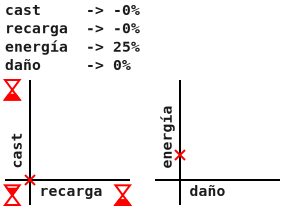
\includegraphics[width=.35\textwidth]{assets/lvl-design/oz.png}
  \end{center}

\item \textbf{Fusil}
  

  \begin{center}
    \begin{tabular}{c|c}
      \textbf{Fortalezas} & \textbf{Debilidades} \\
      \hline
      Caballería & Artillero \\
      Milicia & Munición limitada \\
      Soldado
    \end{tabular}
  \end{center}

  \begin{center}
    \includegraphics[width=.35\textwidth]{assets/lvl-design/fusil.png}
  \end{center}
\end{itemize}

    \paragraph{Diseño de niveles}

  \textit{Advertencia: }El arte usado para el diseño de niveles no es definitivo. Es solo una maqueta

  \paragraph{Especificaciones necesarias}

  \begin{itemize}

  \item \textbf{Duración }Al jugador debería tomarle 13 minutos pasar este nivel.
    \begin{itemize}
    \item \textbf{Batallas} El 60\% de este tiempo, debería tener enemigos presentes en la pantalla. (6 minutos)
    \item \textbf{Explorando} El 20\%, el jugador, probablemente, lo pase experimentando con los comandos, y observando detalles sin avanzar en el mapa. (2.25 minutos).
    \item \textbf{Caminando} El resto del tiempo (20\%), el jugador pasará, probablemente, avanzando hacia la derecha. (casi 6 minutos)
    \end{itemize}
  \item \textbf{Velocidad} Omar Quispe camina a una velocidad de $70\frac{px}{s}$
  \item \textbf{Longitud } Por lo tanto, el juego debería poder pasarse caminando, sin enemigos, en $(15)(60\%) = 9$ minutos. En vista de la velocidad de Omar Quispe, la longitud del juego debería ser de $d = vt = 70 * (9*60) = 10920 px$. Debido al diseño, se ajustó a $14520$ pixeles de largo.

  \item \textbf{Preguntas: }
    \begin{itemize}
    \item \textbf{¿Qué pasó con los caídos?} El jugador podrá desbloquear esta pregunta al encontrar soldados heridos a lo largo del camino e interactuar con ellos.
    \item \textbf{¿Sembradores en el desierto?} Esta pregunta se desbloquea mientras Ladislao está dando su discurso, el jugador podrá ver entre la milicia a algunos granjeros con azadas, las azadas son importantes porque implican que los granjeros no cuidan ganado, sino sembradíos.
    \item \textbf{¿Por qué era estratégicamente importante Calama?} Esta pregunta se desbloquea si el jugador logra sobrevivir hasta el final del nivel.
    \end{itemize}    

  \end{itemize}

  \paragraph{Nivel}

  En La parte inicial, el jugador permanece inmóvil, ya está equipado con una picota, y puede ver a sus compatriotas armados con armas improvisadas, algunos de ellos tienen fusiles.

  Aquí se desarrolla el script.
  \begin{center}
    \includegraphics[width=.9\textwidth]{../prototype/01.png}
  \end{center}

  En la parte inicial, se le enseña al jugador los controles básicos: caminar, correr, la mecánica de la energía y cómo recargarla, y la mecánica de la vida y cómo recargarla.
  \begin{center}
    \includegraphics[width=.9\textwidth]{../prototype/02.png}
  \end{center}


  En la primera batalla se le enseña cómo atacar y cubrirse. Un poco más adelante el jugador consigue la Oz, junto con la pregunta: ¿Sembradores en el desierto?, descubrirá que la oz es más rápida y consume menos energía, pero hace tan poco daño que es difícil acabar con los artilleros con ella. Decidirá si seguir usando su picota, o usar la oz, o una mezcla.
  \begin{center}
    \includegraphics[width=.9\textwidth]{../prototype/03.png}
  \end{center}

  El primer encuentro con la milicia, está diseñado para que el jugador recuerde el funcionamiento de la oz, e intente usarla de nuevo, dándose cuenta que es efectiva contra este tipo de enemigos, pero que la picota es muy difícil de usar contra blancos móviles.
  \begin{center}
    \includegraphics[width=.9\textwidth]{../prototype/04.png}
  \end{center}

  
  El primer encuentro con la caballería, está diseñado para que el jugador se de cuenta que puede esconderse de las batallas. Esta caballería es extremadamente difícil de derrotar con oz o con picota, pero no es imposible. El jugador puede decidir si esconderse, o luchar y terminar sumamente exhausto y herido.

  \begin{center}
    \includegraphics[width=.9\textwidth]{../prototype/05.png}
  \end{center}

  Más adelante, encontrará la lanza, que es ideal contra caballería. Luego, un campo abierto en el que no podrá esconderse, y deberá enfrentarse a la tropa montada con su lanza. Puede enfrentarlo con las otras armas, pero estará demasiado exhausto para hacerlo, así que será muy difícil.
  \begin{center}
    \includegraphics[width=.9\textwidth]{../prototype/06.png}
  \end{center}

  El resto del nivel, transcurre mezclando astutamente estos 4 diferentes tipos de enemigos para que el jugador haga uso de sus habilidades para derrotarlos.

  Y por último, el jugador debería asustarse al ver tantos soldados caídos, durante todo el nivel, la cantidad de soldados caídos es proporcional a la dificultad de la siguiente batalla.

  El jugador tiene la opción de esconderse, o de seguir. Debería darse cuenta que algo anda mal al ver algunos soldados caídos que parecían estar huyendo de la batalla, y más adelante, ve a 3 de ellos corriendo hacia el lado contrario, gritando ``retirada!''. El jugador también tiene la opción de huir, pero no deberá dejar que el fuego enemigo le llegue.x
  
  \begin{center}
    \includegraphics[width=.9\textwidth]{../prototype/07.png}
  \end{center}


  


\end{subsubsection}


\end{subsection}
